\documentclass[a4paper,14pt]{extarticle}

\usepackage[utf8x]{inputenc}
\usepackage[T1]{fontenc}
\usepackage[russian]{babel}
\usepackage{hyperref}
\usepackage{indentfirst}
\usepackage{here}
\usepackage{array}
\usepackage{graphicx}
\usepackage{grffile}
\usepackage{caption}
\usepackage{subcaption}
\usepackage{chngcntr}
\usepackage{amsmath}
\usepackage{amssymb}
\usepackage{pgfplots}
\usepackage{pgfplotstable}
\usepackage[left=2cm,right=2cm,top=2cm,bottom=2cm,bindingoffset=0cm]{geometry}
\usepackage{multicol}
\usepackage{multirow}
\usepackage{titlesec}
\usepackage{listings}
\usepackage{color}
\usepackage{longtable}
\usepackage{enumitem}
\usepackage{cmap}
\usepackage{tikz}

\usetikzlibrary{shapes,arrows}

\definecolor{green}{rgb}{0,0.6,0}
\definecolor{gray}{rgb}{0.5,0.5,0.5}
\definecolor{purple}{rgb}{0.58,0,0.82}

\lstset{
	language={SQL},
	inputpath={../},
	backgroundcolor=\color{white},
	commentstyle=\color{green},
	keywordstyle=\color{blue},
	numberstyle=\scriptsize\color{gray},
	stringstyle=\color{purple},
	basicstyle=\small,
	breakatwhitespace=false,
	breaklines=true,
	captionpos=b,
	keepspaces=true,
	numbers=left,
	numbersep=5pt,
	showspaces=false,
	showstringspaces=false,
	showtabs=false,
	tabsize=8,
	frame=single,
}

\renewcommand{\le}{\ensuremath{\leqslant}}
\renewcommand{\leq}{\ensuremath{\leqslant}}
\renewcommand{\ge}{\ensuremath{\geqslant}}
\renewcommand{\geq}{\ensuremath{\geqslant}}
\renewcommand{\epsilon}{\ensuremath{\varepsilon}}
\renewcommand{\phi}{\ensuremath{\varphi}}
\renewcommand{\thefigure}{\arabic{figure}}
\def\code#1{\texttt{#1}}

\titleformat*{\section}{\large\bfseries} 
\titleformat*{\subsection}{\normalsize\bfseries} 
\titleformat*{\subsubsection}{\normalsize\bfseries} 
\titleformat*{\paragraph}{\normalsize\bfseries} 
\titleformat*{\subparagraph}{\normalsize\bfseries} 

\counterwithin{figure}{section}
\counterwithin{equation}{section}
\counterwithin{table}{section}
\newcommand{\sign}[1][5cm]{\makebox[#1]{\hrulefill}}
\newcommand{\equipollence}{\quad\Leftrightarrow\quad}
\newcommand{\no}[1]{\overline{#1}}
\graphicspath{{../}}
\captionsetup{justification=centering,margin=1cm}
\def\arraystretch{1.3}
\setlength\parindent{5ex}
\titlelabel{\thetitle.\quad}

\setitemize{itemsep=0em}
\setenumerate{itemsep=0em}

\tikzstyle{startstop} = [
	rectangle,
	align=center,
	rounded corners,
	text width=10em,
	text centered,
	draw=black
]
\tikzstyle{process} = [
	rectangle,
	align=center,
	text width=20em,
	text centered,
	draw=black
]
\tikzstyle{decision} = [
	diamond,
	aspect=4,
	align=center,
	inner sep=0pt,
	text width=10em,
	text centered,
	node distance=5em,
	draw=black
]
\tikzstyle{line} = [
	draw=black,
	thick,
	->,
	>=stealth,
	-latex'
]

\begin{document}

\begin{titlepage}
\begin{center}
	САНКТ-ПЕТЕРБУРГСКИЙ ПОЛИТЕХНИЧЕСКИЙ УНИВЕРСИТЕТ\\ ПЕТРА ВЕЛИКОГО\\[0.3cm]
	\par\noindent\rule{10cm}{0.4pt}\\[0.3cm]
	Институт компьютерных наук и технологий \\[0.3cm]
	Кафедра компьютерных систем и программных технологий\\[4cm]
	
	Отчет по лабораторной работе № 1\\[3mm]
	Дисциплина: <<Базы данных>>\\[3mm]
	Тема: <<Разработка структуры БД>>\\[7cm]
\end{center}

\begin{flushleft}
	\hspace*{5mm} Выполнил студент гр. 43501/3  \hspace*{2.5cm}\sign[3cm]\hspace*{3.0mm} А.Ю. Ламтев\\
	\hspace*{10.4cm} (подпись)\\[3mm]
	\hspace*{5mm} Преподаватель \hspace*{6.0cm}\sign[3cm]\hspace*{2mm} А.В. Мяснов\\
	\hspace*{10.4cm} (подпись)\\[3mm]
	\hspace*{11.1cm} <<\sign[7mm]>> \sign[27mm] \the\year\hspace{1mm} г.
\end{flushleft}

\vfill

\begin{center}
	Санкт-Петербург\\
	\the\year
\end{center}
\end{titlepage}
\addtocounter{page}{1}

\tableofcontents
\newpage

\section{Цели работы}

Сформировать набор данных, позволяющий производить операции на реальных объемах данных. 

\section{Программа работы}

\begin{enumerate}
	\item Реализация в виде программы параметризуемого генератора, который позволит сформировать набор связанных данных в каждой таблице.
	\item Частные требования к генератору, набору данных и результирующему набору данных:
	\begin{itemize}
		\item количество записей в справочных таблицах должно соответствовать ограничениям предметной области
		\item количество записей в таблицах, хранящих информацию об объектах или субъектах должно быть параметром генерации
		\item значения для внешних ключей необходимо брать из связанных таблиц
	\end{itemize}
 
\end{enumerate}
 
\section{Разработка генератора} 

Генератор выполнен в виде консольного приложения, разработанного на языке \code{Java} последней версии \code{11.0.1}. Программа ожидает 3 аргумента командной строки: путь к файлу в формате \code{json}, в котором содержатся \code{url} \code{Postgres}-сервера, и имя пользователя, и пароль для доступа к нему; и путь к файлу в формате \code{json}, содержащему параметры генератора (обязательные параметры); и значение из множества \code{\{onlyMovies, onlySeries, onlyUsers, onlyMovieSubscriptions, onlySeriesSubscriptions\}}, которое позволяет догенерировать определённые данные (если этот аргумент отсутствует, то генерируются данные для всех таблиц). Примеры этих 2-х файлов представлены в листингах \ref{lst:db.json} и \ref{lst:params.json}.

\begin{lstlisting}[label={lst:db.json},caption={Пример параметров доступа к \code{Postgres}-серверу}]
{
  "url": "jdbc:postgresql://localhost:5432/postgres",
  "user": "postgres",
  "password": "postgres"
}
\end{lstlisting}

\lstinputlisting[caption={Пример параметров генератора},label={lst:params.json}]{params.json}

Рассмотрим подробнее параметры генератора:

\begin{itemize}
	\item \code{usersCount} --- число пользователей
	\item \code{femalePercentage} --- процент девушек от общего числа пользователей
	\item \code{moviesCount} --- число самостоятельных фильмов (эпизоды сериалов в это число не входят)
	\item \code{seriesCountSeasonsEpisodes} --- массив типов сериалов, параметризуемый 3-мя значениями: числом сериалов данного типа, числом сезонов в таких сериалах и количество серий в каждом сезоне (\code{[100, 3, 15]} означает 100 сериалов, в каждом 3 сезона, состоящих из 15 серий)
	\item \code{percentageOfUsersWhoBoughtMovies} --- процент пользователей, купивших хотя бы 1 фильм на постоянной основе.
	\item \code{minMoviesPerUser} --- минимальное число фильмов, которые купил пользователь, входящий в группу, описываемую предыдущим параметром.
	\item \code{maxMoviesPerUser} --- аналогично предыдущему параметру -- максимальное число фильмов.
	\item \code{percentageOfUsersWhoBoughtSeries} --- процент пользователей, купивших хотя бы 1 сериал на постоянной основе.
	\item \code{minSeriesPerUser} --- минимальное число сериалов, которые купил пользователь, входящий в группу, описываемую предыдущим параметром.
	\item \code{maxSeriesPerUser} --- аналогично предыдущему параметру -- максимальное число сериалов
	\item \code{yearsSinceFirstSubscription} --- число лет, прошедших с первой подписки
	\item \code{minSubscriptionsPerUser} --- минимальное число подписок у пользователя
	\item \code{maxSubscriptionsPerUser} --- максимальное число подписок у пользователя
	\item \code{moviesSubscriptionsPercentage} --- процент подписок на фильмы от общего числа подписок (на фильмы и сериалы)
	\item \code{durationPriceNMoviesMSeasons} --- массив типов подписок, параметризуемый 4-мя значениями: длительностью в днях, стоимостью в \$, соответствующему числу фильмов и соответствующему числу сезонов сериалов (\code{[90, 35, 15, 3]} означает, что подписка на 90 дней, стоимостью \$35, и в неё входят либо 15 фильмов, либо 3 сериала).


Для соединения с базой данных используется \code{JDBC} драйвер последней версии \code{42.2.5}.

В качестве системы сборки и управления зависимостями проекта выбран \code{Gradle} версии \code{5.0}, конфигурационные файлы проекта написаны на \code{Kotlin DSL}. Они представлены в листингах \ref{lst:build} и \ref{lst:settings}.

\lstinputlisting[caption={build.gradle.kts},label={lst:build},language={Scala}]{build.gradle.kts}

\lstinputlisting[caption={settings.gradle.kts},label={lst:settings},language={Scala}]{settings.gradle.kts}
	
\end{itemize}

Приложение логически разделено на 2 части:

\begin{enumerate}
	\item \textbf{Обработка аргументов командной строки и парсинг конфигурационных файлов}\\
	
	Состоит из класса \code{ArgumentsParser} с бизнес-логикой, исходный код которого приведён в листинге \ref{lst:ArgumentsParser}. А также классов \code{EndpointInfo} (листинг \ref{lst:EndpointInfo}) и \code{Parameters} (листинг \ref{lst:Parameters}), которые являются моделью для входных \code{json} файлов.
	
	Для десериализации \code{json} файлов в объекты классов используется библиотека \code{Gson}.	
	
	\item \textbf{Генерация данных и заполнение ими БД}\\
	
	На рис. \ref{fig:movie-service-diagram} представлена схема БД, состоящей из 16 таблиц.
	
	\begin{figure}[H]
		\centering
		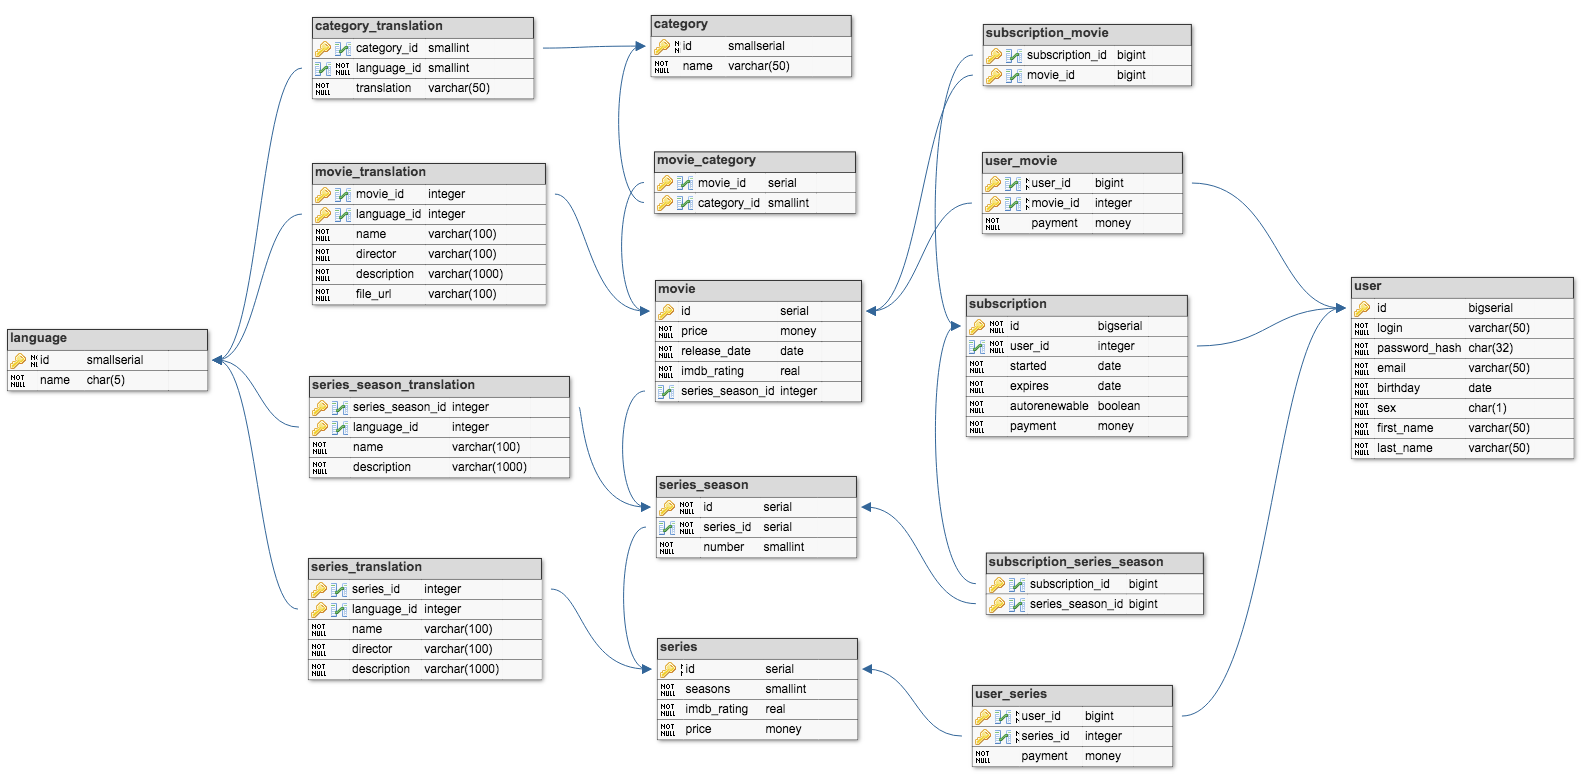
\includegraphics[width=1.0\textwidth]{../../lab2/diagrams/movie-service-diagram}
		\caption{Cхема БД}
		\label{fig:movie-service-diagram}
	\end{figure}
	
	Для заполнения соответствующих таблиц были разработаны классы, реализующие интерфейс \code{TableGenerator} (листинг \ref{lst:TableGenerator}):
	
	\begin{itemize}
		\item \code{LanguageTableGenerator} (листинг \ref{lst:LanguageTableGenerator}) --- генератор данных для таблицы \code{language}
		\item \code{CategoryTableGenerator} (листинг \ref{lst:CategoryTableGenerator})  --- генератор данных для таблицы \code{category}
		\item \code{CategoryTranslationTableGenerator} (листинг \ref{lst:CategoryTranslationTableGenerator})  --- генератор данных для таблицы \code{category\_translation}
		\item \code{MovieTableGenerator} (листинг \ref{lst:MovieTableGenerator})  --- генератор данных для таблицы \code{movie}
		\item \code{MovieTranslationTableGenerator} (листинг \ref{lst:MovieTranslationTableGenerator})  --- генератор данных для таблицы \code{movie\_translation}
		\item \code{MovieCategoryTableGenerator} (листинг \ref{lst:MovieCategoryTableGenerator})  --- генератор данных для таблицы \code{movie\_category}
		\item \code{SeriesTableGenerator} (листинг \ref{lst:SeriesTableGenerator})  --- генератор данных для таблицы \code{series}
		\item \code{SeriesTranslationTableGenerator} (листинг \ref{lst:SeriesTranslationTableGenerator})  --- генератор данных для таблицы \code{series\_translation}
		\item \code{SeriesSeasonTableGenerator} (листинг \ref{lst:SeriesSeasonTableGenerator})  --- генератор данных для таблицы \code{series\_season}
		\item \code{SeriesSeasonTranslationTableGenerator} (листинг \ref{lst:SeriesSeasonTranslationTableGenerator})  --- генератор данных для таблицы \code{series\_season\_translation}
		\item \code{UserTableGenerator} (листинг \ref{lst:UserTableGenerator})  --- генератор данных для таблицы \code{user}
		\item \code{UserMovieTableGenerator} (листинг \ref{lst:UserMovieTableGenerator})  --- генератор данных для таблицы \code{user\_movie}
		\item \code{UserSeriesTableGenerator} (листинг \ref{lst:UserSeriesTableGenerator})  --- генератор данных для таблицы \code{user\_series}
		\item \code{SubscriptionTableGenerator} (листинг \ref{lst:SubscriptionTableGenerator})  --- генератор данных для таблицы \code{subscription}
		\item \code{SubscriptionMovieTableGenerator} (листинг \ref{lst:SubscriptionMovieTableGenerator})  --- генератор данных для таблицы \code{subscription\_movie}
		\item \code{SubscriptionSeriesSeasonTableGenerator} (листинг \ref{lst:SubscriptionSeriesSeasonTableGenerator})  --- генератор данных для таблицы \code{subscription\_series\_season}
	\end{itemize}
	
	При формировании новых данных иногда требовались данные, уже содержащиеся в таблицах (в частности, значения внешних ключей). Для извлечения из БД этих данных было разработано 2 класса: 
	
	\begin{itemize}
		\item \code{StorageDAO} (листинг \ref{lst:StorageDAO}) --- класс, в котором реализованы \code{SELECT} запросы к базе данных, позволяющие получить число записей в произвольной таблице или получить все первичные ключи таблицы.
		\item \code{SubscriptionTableDAO} (листинг \ref{lst:SubscriptionTableDAO}) --- класс, в котором реализован \code{SELECT} запрос, специфичный только для таблицы \code{subscription}.
	\end{itemize}
	
	Также был разработан утилитный класс \code{Utils} (листинг \ref{lst:Utils}), в котором реализованы вспомогательные функциональности, используемые при генерации данных для разных таблиц.
	
	Для генерации различных данных, таких, как названия фильмов, сериалов, имена пользователей, даты и т.д. использовалась библиотека \code{JavaFaker}.
	
\end{enumerate}

\section{Выводы}

В результате работы был разработан параметризуемый генератор, с помощью которого БД была заполнена данными. Эти данные состоят из десятков тысяч пользователей; десятков тысяч фильмов; тысяч сериалов, содержащих, десятки тысяч серий; сотен тысяч подписок...

Также был получен опыт организации взаимодействия \code{Java}-приложений с базами данных с помощью стандарта \code{JDBC}.

\section*{Приложение 1. Исходный код}
\addcontentsline{toc}{section}{Приложение 1. Исходный код}

\lstinputlisting[caption={Launcher.java},label={lst:Launcher},language={Java}]{src/main/java/com/lamtev/movie_service/datagen/Launcher.java}

\lstinputlisting[caption={ArgumentsParser.java},label={lst:ArgumentsParser},language={Java}]{src/main/java/com/lamtev/movie_service/datagen/cli_args/ArgumentsParser.java}

\lstinputlisting[caption={EndpointInfo.java},label={lst:EndpointInfo},language={Java}]{src/main/java/com/lamtev/movie_service/datagen/cli_args/EndpointInfo.java}

\lstinputlisting[caption={Parameters.java},label={lst:Parameters},language={Java}]{src/main/java/com/lamtev/movie_service/datagen/cli_args/Parameters.java}

\lstinputlisting[caption={TableGenerator.java},label={lst:TableGenerator},language={Java}]{src/main/java/com/lamtev/movie_service/datagen/generator/TableGenerator.java}

\lstinputlisting[caption={LanguageTableGenerator.java},label={lst:LanguageTableGenerator},language={Java}]{src/main/java/com/lamtev/movie_service/datagen/generator/LanguageTableGenerator.java}

\lstinputlisting[caption={CategoryTableGenerator.java},label={lst:CategoryTableGenerator},language={Java}]{src/main/java/com/lamtev/movie_service/datagen/generator/category/CategoryTableGenerator.java}

\lstinputlisting[caption={CategoryTranslationTableGenerator.java},label={lst:CategoryTranslationTableGenerator},language={Java}]{src/main/java/com/lamtev/movie_service/datagen/generator/category/CategoryTranslationTableGenerator.java}

\lstinputlisting[caption={MovieTableGenerator.java},label={lst:MovieTableGenerator},language={Java}]{src/main/java/com/lamtev/movie_service/datagen/generator/movie/MovieTableGenerator.java}

\lstinputlisting[caption={MovieTranslationTableGenerator.java},label={lst:MovieTranslationTableGenerator},language={Java}]{src/main/java/com/lamtev/movie_service/datagen/generator/movie/MovieTranslationTableGenerator.java}

\lstinputlisting[caption={MovieCategoryTableGenerator.java},label={lst:MovieCategoryTableGenerator},language={Java}]{src/main/java/com/lamtev/movie_service/datagen/generator/movie/MovieCategoryTableGenerator.java}

\lstinputlisting[caption={SeriesTableGenerator.java},label={lst:SeriesTableGenerator},language={Java}]{src/main/java/com/lamtev/movie_service/datagen/generator/series/SeriesTableGenerator.java}

\lstinputlisting[caption={SeriesTranslationTableGenerator.java},label={lst:SeriesTranslationTableGenerator},language={Java}]{src/main/java/com/lamtev/movie_service/datagen/generator/series/SeriesTranslationTableGenerator.java}

\lstinputlisting[caption={SeriesSeasonTableGenerator.java},label={lst:SeriesSeasonTableGenerator},language={Java}]{src/main/java/com/lamtev/movie_service/datagen/generator/series/season/SeriesSeasonTableGenerator.java}

\lstinputlisting[caption={SeriesSeasonTranslationTableGenerator.java},label={lst:SeriesSeasonTranslationTableGenerator},language={Java}]{src/main/java/com/lamtev/movie_service/datagen/generator/series/season/SeriesSeasonTranslationTableGenerator.java}

\lstinputlisting[caption={UserTableGenerator.java},label={lst:UserTableGenerator},language={Java}]{src/main/java/com/lamtev/movie_service/datagen/generator/user/UserTableGenerator.java}

\lstinputlisting[caption={UserMovieTableGenerator.java},label={lst:UserMovieTableGenerator},language={Java}]{src/main/java/com/lamtev/movie_service/datagen/generator/user/UserMovieTableGenerator.java}

\lstinputlisting[caption={UserSeriesTableGenerator.java},label={lst:UserSeriesTableGenerator},language={Java}]{src/main/java/com/lamtev/movie_service/datagen/generator/user/UserSeriesTableGenerator.java}

\lstinputlisting[caption={SubscriptionTableGenerator.java},label={lst:SubscriptionTableGenerator},language={Java}]{src/main/java/com/lamtev/movie_service/datagen/generator/subscription/SubscriptionTableGenerator.java}

\lstinputlisting[caption={SubscriptionMovieTableGenerator.java},label={lst:SubscriptionMovieTableGenerator},language={Java}]{src/main/java/com/lamtev/movie_service/datagen/generator/subscription/SubscriptionMovieTableGenerator.java}

\lstinputlisting[caption={SubscriptionSeriesSeasonTableGenerator.java},label={lst:SubscriptionSeriesSeasonTableGenerator},language={Java}]{src/main/java/com/lamtev/movie_service/datagen/generator/subscription/SubscriptionSeriesSeasonTableGenerator.java}

\lstinputlisting[caption={StorageDAO.java},label={lst:StorageDAO},language={Java}]{src/main/java/com/lamtev/movie_service/datagen/generator/StorageDAO.java}

\lstinputlisting[caption={SubscriptionTableDAO.java},label={lst:SubscriptionTableDAO},language={Java}]{src/main/java/com/lamtev/movie_service/datagen/generator/subscription/SubscriptionTableDAO.java}

\lstinputlisting[caption={Utils.java},label={lst:Utils},language={Java}]{src/main/java/com/lamtev/movie_service/datagen/generator/Utils.java}

\end{document}
